\section{Experiments}
Our goal was to reproduce the main experiment in~\cite{Kipf2016}, and also, perform our own experiment and compare our results. We followed the model proposed in the paper, but instead of using the tensorflow framework, we used pytorch framework.

\subsection{The Model}
The model utilized by the authors' is a 2-layer convolution network, and it can be represented by Equation \ref{Equation1} and Figure \ref{fig:model} illustrates the set up.

\begin{equation}
    \label{Equation1}
    Z = f(x,A) = softmax(\hat{A}ReLU(\hat{A}XW_{0})W_{1}) 
\end{equation}

\begin{figure}[h!]
  \centering
  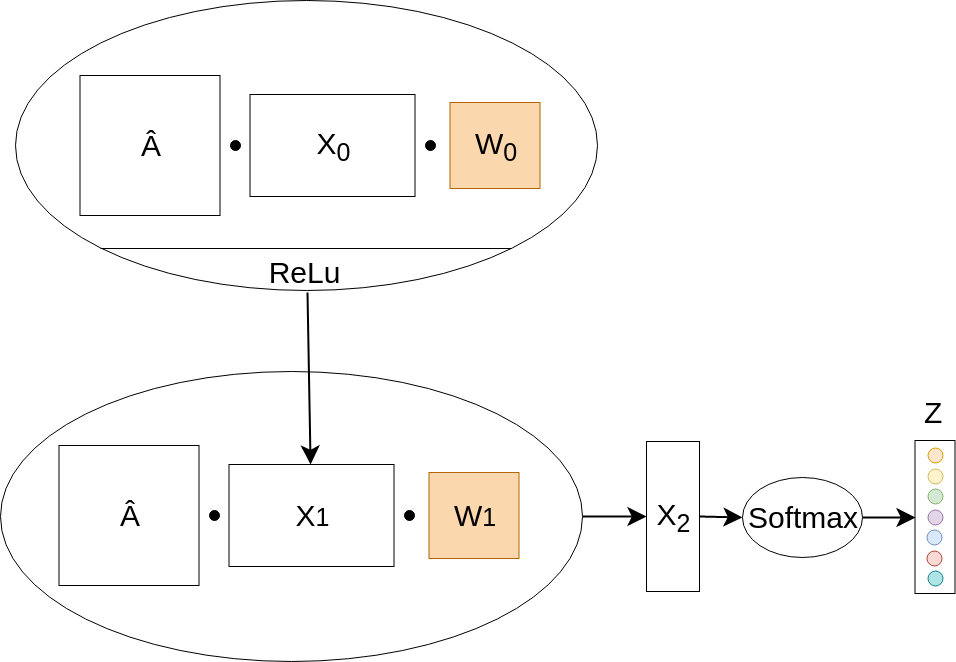
\includegraphics[width=0.75\linewidth]{media/model_right.png}
  
  \caption{Graph Convolution Network}
  \label{fig:model}
\end{figure}

The pass forward works where the first layer takes as input a matrix $x_{0}$ that contains the features of the data. This matrix is used to calculate the dot product with the \textit{normalized adjacency matrix} $\hat{A}$ and the weight matrix $w_{0}$. After the dot product is done the result is passed through the \textit{RelU}activation function, and the result matrix is used as input $x_{1}$ for layer 2.

In layer 2, $x_{1}$ that comes from layer one is used to calculate the dot product with the same \textit{normalized adjacency matrix} and a matrix of weights $w_{1}$.

The matrix generated by the second matrix is passed through a \textit{softmax} so the data can be classified into the classes.


\subsection{Datasets}

Following the experiments of ~\cite{Kipf2016}, we used 3 of their 4 datasets from citation networks: Cora, Citesser and Pubmed. The three datasets are set up where the nodes are papers (documents) and the edges are citation links. In Table ~\ref{tab:datasets} we have the datasets statistics. Training can only be done in nodes that have labels, in our case there are 20 nodes per class for each dataset, the total number per dataset is shown in the trainable nodes column.

\begin {table}[ht]
  \begin{center}
    \begin{tabular}{|c|c|c|c|c|}
    \hline
    Dataset  & Nodes  & Classes & Features & Trainable nodes\\
    \hline 
    Cora     & 2,708  & 7       & 1,433    & 140 \\ 
    Citeseer & 3,327  & 6       & 3,703    & 120  \\  
    Pubmed   & 19,717 & 3       & 500      & 60   \\
    \hline
    \end{tabular}
  \end{center}
\caption {Datasets} \label{tab:datasets} 
\end{table}

\subsection{Experiment 1}

We reproduced the authors' experiment with the hyperparameters presented in Table \ref{tab:hyperparameters1}.

\begin {table}[ht]
  \begin{center}
    \begin{tabular}{|c|c|}
    \hline
    Learning rate     & 0.01 \\ 
    Epochs            & 200  \\ 
    Optimization      & ADAM \\
    Drop out          & 0.5   \\
    Weight Decay      & 0.0005 \\
    Regularization    & L2    \\
    Hidden Features   & 16    \\
    \hline
    \end{tabular}
  \end{center}
\caption {Hyperparameters Experiment 1} \label{tab:hyperparameters1} 
\end{table}

 The results for this experiment are described in Table \ref{tab:results1}.

\begin {table}[ht]
  \begin{center}
    \begin{tabular}{|c|c|c|c|c|}
    \hline
    Dataset    &  Training Accuracy & Validation Accuracy & Testing Accuracy & Paper Test Accuracy \\ \hline
    Cora          & 99.43 \% & 73.80 \%  & 81.05 \% & 81.50 \% \\ 
    Citesser      & 94.92 \% & 62.84 \%  & 71.70 \% & 70.30 \% \\
    Pubmed        & 98.67 \% & 76.28 \%  & 80.00 \% & 79.00 \% \\
    \hline
    \end{tabular}
  \end{center}
\caption {Results Experiment 1} \label{tab:results1} 
\end{table}

From the results in Table \ref{tab:results1} for Validation Accuracy, it is clear that overfitting is a problem in this experiment, since the training set is very small, the entire model is only trained on the labeled nodes, therefore there is low generalization. For this same reason, we get very high Training Accuracy. 

\subsection{Experiment 2}
In experiment 2, we trained the Cora dataset and fine tuned our own hyperparameters as presented in Table \ref{tab:hyperparameters2}.

\begin {table}[ht]
  \begin{center}
    \begin{tabular}{|c|c|}
    \hline
    Learning rate     & 0.012 \\ 
    Epochs            & 200  \\ 
    Optimization      & ADAM \\
    Drop out          & 0.64   \\
    Weight Decay      & 0.0006 \\
    Regularization    & L2    \\
    Hidden Features   & 102   \\
    \hline
    \end{tabular}
  \end{center}
\caption {Hyperparameters Experiment 2} \label{tab:hyperparameters2} 
\end{table}

The results for Experiment 2 are presented in Table.

\begin {table}[ht]
  \begin{center}
    \begin{tabular}{|c|c|c|c|}
    \hline
    Dataset    &  Training Accuracy & Validation Accuracy & Testing Accuracy\\ \hline
    Cora          & 98.57 \% & 75.80 \%  & 81.80 \% \\ 
    Citesser      & 100.00 \%& 67.20 \%  & 71.20 \% \\
    Pubmed        & 100.00 \%& 77.80 \%  & 79.30 \% \\
    \hline
    \end{tabular}
  \end{center}
\caption {Results Experiment 2} \label{tab:results2} 
\end{table}

The same behavior for Validation and Training Accuracy were observed in this experiment.

\subsection{Loss}

The loss function for this experiment is the standard \textit{cross-entropy loss} and it is represented by Equation \ref{loss}.

\begin{equation}
  \label{loss}
  \mathcal{L} = - \sum_{l \in \mathcal{Y}_{L}} \sum_{f=1}^{F} Y_{lf}lnZ_{lf}  
\end{equation}

Where Y represents the ground truth and Z the predictions. Just as the training the loss, is also calculated on the subset of the nodes that were labeled. Our results for loss are described in Tables \ref{tab:loss1} and \ref{tab:loss2}.

\begin {table}[ht]
\parbox{.45\linewidth}{
\begin{center}
  \begin{tabular}{|c|c|}
  \hline
  Dataset       &  Loss\\ \hline
  Cora          & 0.7964997291564941 \\ 
  Citesser      & 0.9455778002738953 \\
  Pubmed        & 0.5608009696006775 \\
  \hline
  \end{tabular}
\end{center}
\caption {Loss Experiment 1} \label{tab:loss1} 
}
\hfill
\parbox{.45\linewidth}{
\begin{center}
  \begin{tabular}{|c|c|}
  \hline
  Dataset       &  Loss\\ \hline
  Cora          & 0.7033339738845825 \\ 
  Citesser      & 0.9455778002738953 \\
  Pubmed        & 0.5608009696006775 \\
  \hline
  \end{tabular}
\end{center}
\caption {Loss Experiment 2} \label{tab:loss2} 
}
\end{table}

The original paper in which our work was based on did not present any values for loss in their experiments.